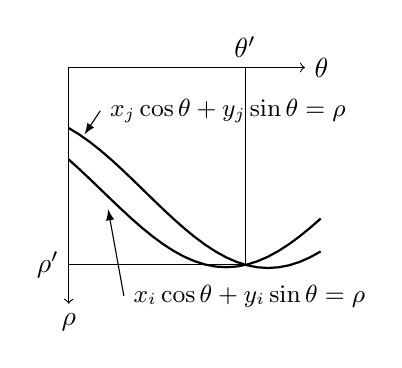
\begin{tikzpicture}[domain=0:3.2]
	% Koordinatensystem
	\draw[->] (0,0) -- +(3,0) node[right] {$\theta$};
	\draw[->] (0,0) -- +(0,-3) node[below] {$\rho$};
	% Kurven + Beschriftung
	% Die Kurven müssen etwas zurechtgestaucht werden, damit auch alles richtig passt. Ansosnten enprechen sie der richtigen Transfromation.
	\draw[thick] plot(\x, { -(3.14/2) + 0.4*(2.2 *cos( (\x + (3.14/2) ) r) + sin( (\x + (3.14/2) ) r)) });
	\draw[thick] plot(\x, { -(3.14/2) + 0.4*(1.4 *cos( (\x + (3.14/2) ) r) + 2* sin( (\x + (3.14/2) ) r)) });
	\draw[latex-] (0.2,-0.85) -- +(0.2,0.3) node[right] {\small $x_j\cos\theta + y_j\sin\theta = \rho$} ;
	\draw[latex-] (0.5,-1.8) -- +(0.2,-1.1) node[right] {\small $x_i\cos\theta + y_i\sin\theta = \rho$} ;
	% Schnittpunk der Geraden mit Beschriftung
	\draw (2.24,0) -- ++(0,-2.5) -- +(-2.24,0);
	\node[above] at (2.24, 0) {$\theta'$};
	\node[left] at (0, -2.5) {$\rho'$};
\end{tikzpicture}